\documentclass[aspectratio=169]{beamer}

%%% Обязательные пакеты
%% Beamer
\usepackage{beamerthemesplit}
\usetheme{SPbGU}
\beamertemplatenavigationsymbolsempty
\usepackage{appendixnumberbeamer}

%% Локализация
\usepackage{fontspec}
% Используем системные шрифты macOS
\setmainfont{Times New Roman}
\setsansfont{Helvetica Neue}
\setmonofont{Menlo}

\usepackage{polyglossia}
\setdefaultlanguage{russian}
\setotherlanguage{english}
\usepackage[autostyle]{csquotes}

%% Графика
\usepackage{wrapfig}
\usepackage{pdfpages}

%% Математика
\usepackage{amsmath, amsfonts, amssymb, amsthm, mathtools}

%% Дополнительные пакеты
\usepackage{tikz}
\usetikzlibrary{decorations.pathreplacing,calc,shapes,positioning,tikzmark}

\usepackage{multirow}
\usepackage{fancyvrb}


% Кириллические fallback'и для polyglossia (Helvetica Neue не содержит кириллицу)
\newfontfamily\cyrillicfont{Times New Roman}
\newfontfamily\cyrillicfontsf{PT Sans}
\newfontfamily\cyrillicfonttt{Menlo}

\usepackage{booktabs}
\usepackage{array}

\title[Дообучение YandexGPT]{Анализ влияния дообучения YandexGPT \\ на корректность выбора функции \\ для получения данных по исходному запросу}
\institute[СПбГУ]{}
\author[Горошко А.\,В.]{Горошко Андрей Витальевич, группа 22.Б13-мм}
\date{2026}

\begin{document}

%% =========================================================
%% 1. Титул
%% =========================================================
{
\setbeamertemplate{footline}{}
\begin{frame}
  
\includegraphics[width=1.2cm]{pictures/SPbGU_Logo.png}
  \vspace{-28pt}\hspace{-10pt}
  \begin{center}
    \begin{tabular}{c}
      \scriptsize Санкт-Петербургский государственный университет \\
      \scriptsize Кафедра математики и компьютерных наук \\
      \scriptsize 02.03.01 «Математика и компьютерные науки», СВ.5001.2022
    \end{tabular}
    \titlepage
  \end{center}

  \vspace{-12pt}
  {\scriptsize
    \textbf{Научный руководитель:} доц.\ Григорьева~А.~В. \\
    \textbf{Рецензент:} ст.\,преп.\ Севостьянов~Р.~А., к.\,ф.-м.\,н.
  }
  \begin{center}
    \scriptsize Санкт-Петербург, 2026
  \end{center}
\end{frame}
}

%% =========================================================
%% 2. Контекст
%% =========================================================
\begin{frame}
\frametitle{Контекст: AI-агенты и tool use}
\begin{columns}[T]
\begin{column}{0.55\textwidth}
\begin{itemize}
  \item LLM~— ядро современного AI-агента
  \item \textit{Function calling}: модель сама решает, какую функцию вызвать
  \item Прикладная задача~— AI-агент в домене недвижимости
  \item Два инструмента:
    \begin{itemize}
      \item \texttt{ResolveEntities} (GEO)~— города, станции, адреса
      \item \texttt{SearchTags} (TAG)~— характеристики объекта
    \end{itemize}
\end{itemize}

\vspace{0.6em}
\textbf{Ключевое разграничение:}\\
«у~метро~Сокол» $=$ GEO\\
«у~метро» $=$ TAG (категория транспортной доступности)
\end{column}
\begin{column}{0.43\textwidth}
\begin{center}
\begin{tikzpicture}[
  every node/.style={font=\footnotesize},
  box/.style={rectangle, rounded corners, draw=black!60, fill=black!4, minimum width=2.4cm, minimum height=0.6cm, align=center},
  ar/.style={->, >=stealth, thick}
]
  \node[box] (q) {Запрос пользователя};
  \node[box, below=0.55cm of q] (llm) {LLM (YandexGPT)};
  \node[box, below left=0.7cm and -0.4cm of llm] (geo) {ResolveEntities\\\scriptsize GEO};
  \node[box, below right=0.7cm and -0.4cm of llm] (tag) {SearchTags\\\scriptsize TAG};
  \draw[ar] (q) -- (llm);
  \draw[ar] (llm) -- (geo);
  \draw[ar] (llm) -- (tag);
\end{tikzpicture}
\end{center}
\end{column}
\end{columns}
\end{frame}

%% =========================================================
%% 3. Проблема
%% =========================================================
\begin{frame}
\frametitle{Проблема: baseline неприменим в production}
\begin{columns}[T]
\begin{column}{0.55\textwidth}
YandexGPT~5.1~Pro \emph{без дообучения} на benchmark-combined (500 запросов):
\begin{itemize}
  \item Accuracy $= 81{,}8\%$
  \item Macro $F_1 = 0{,}526$
  \item Recall класса TAG $= 49{,}4\%$
  \item Без \texttt{tool\_call}: $\rho_\varnothing = 6{,}8\%$ (34 запроса)
\end{itemize}

\vspace{0.5em}
\textbf{Систематический bias к GEO:}\\
все 57 ошибок одного типа $\mathrm{TAG}\to\mathrm{GEO}$, ни одной обратной.
\end{column}
\begin{column}{0.43\textwidth}
\textbf{Пример ошибки baseline:}

\medskip
\begin{quote}
\itshape
«квартира с панорамными окнами и видом на парк»
\end{quote}

\smallskip
\textbf{Истинно:} \texttt{SearchTags} (TAG)\\
\textbf{Предсказание:} \texttt{ResolveEntities} (GEO)\\
\textbf{Эффект:} агент ищет несуществующий «парк»-топоним, вместо фильтра по характеристике.
\end{column}
\end{columns}
\end{frame}

%% =========================================================
%% 4. Цель и задачи
%% =========================================================
\begin{frame}
\frametitle{Цель и задачи}
\textbf{Цель:} экспериментально проверить, что LoRA-дообучение значимо улучшает корректность выбора функции в AI-агенте.

\bigskip
\textbf{Задачи:}
\begin{enumerate}
  \item Формализовать выбор инструмента как бинарную классификацию; собрать два независимых бенчмарка (combined и real).
  \item Разработать воспроизводимый пайплайн дообучения и оценки (CLI \texttt{ml-benchmark}).
  \item Обучить и оценить 12 конфигураций моделей с вариацией типа и объёма обучающих данных.
  \item Применить строгий статистический анализ (Cochran~$Q$, McNemar, bootstrap).
\end{enumerate}
\end{frame}

%% =========================================================
%% 5. Формальная постановка
%% =========================================================
\begin{frame}
\frametitle{Формальная постановка}
Классификатор первого \texttt{tool\_call}:
\[
  f_\theta\colon \mathcal{X} \to \{t_{\mathrm{GEO}},\; t_{\mathrm{TAG}}\}.
\]
\begin{columns}[T]
\begin{column}{0.5\textwidth}
\textbf{Ошибки:}
\begin{itemize}
  \item \emph{I рода:} $\mathrm{TAG}\!\to\!\mathrm{GEO}$ \\ агент ищет несуществующий гео-объект.
  \item \emph{II рода:} $\mathrm{GEO}\!\to\!\mathrm{TAG}$ \\ теряется географическая привязка.
  \item Третий исход: $\rho_\varnothing$~— модель не сгенерировала вызов инструмента.
\end{itemize}
\end{column}
\begin{column}{0.46\textwidth}
\textbf{Реальные примеры:}
\begin{itemize}
  \item GEO: «снять квартиру в~центре Казани на~месяц»
  \item TAG: «квартира с~панорамными окнами и~видом на~парк»
  \item Спорный (TAG): «возле зелёной ветки» (жаргон)
\end{itemize}
\end{column}
\end{columns}
\end{frame}

%% =========================================================
%% 6. Гипотезы и критерии успеха
%% =========================================================
\begin{frame}
\frametitle{Гипотезы и критерии успеха}
\textbf{H1a (значимость).} Дообучение значимо снижает долю ошибок относительно baseline.\\
\hphantom{aaaa}\emph{Тест:} односторонний McNemar, $\alpha = 0{,}05$.

\smallskip
\textbf{H1b (порог).} Нижняя граница 95\,\% bootstrap-CI accuracy лучшей модели $> 0{,}9$.

\smallskip
\textbf{H2 (качество $>$ объём).} Сбалансированный микс реальных и синтетических данных превосходит чистую синтетику при равном или большем объёме.

\bigskip
\begin{center}
\begin{tabular}{lrrl}
\toprule
\textbf{Метрика} & \textbf{Baseline} & \textbf{Цель} & \textbf{Бенчмарк} \\
\midrule
Accuracy                 & $81{,}8\%$ & $> 90\%$  & combined \\
Macro $F_1$              & $0{,}526$  & $> 0{,}85$ & combined \\
Recall ($t_{\mathrm{TAG}}$) & $49{,}4\%$ & $> 75\%$ & combined \\
$\rho_\varnothing$       & $6{,}8\%$  & $< 3\%$    & combined \\
\bottomrule
\end{tabular}
\end{center}
\end{frame}

%% =========================================================
%% 7. Гипотеза поверхностного выравнивания
%% =========================================================
\begin{frame}
\frametitle{Гипотеза поверхностного выравнивания (SAH)}
\textbf{LIMA, Zhou et al.\ (2023):}
\begin{quote}
Knowledge is learnt during pretraining; alignment teaches the model \emph{which subdistribution of formats} to use.
\end{quote}

\textbf{Аналогия для tool selection:}\\
выбор функции~— устойчивый \emph{паттерн формы ответа}, а не семантическое знание.\\
Соответственно, небольшого набора качественных примеров достаточно для радикального улучшения.
\end{frame}

%% =========================================================
%% 8. Положение в литературе
%% =========================================================
\begin{frame}
\frametitle{Положение в литературе}
\begin{columns}[T]
\begin{column}{0.48\textwidth}
\textbf{Дообучение:}
\begin{itemize}
  \item LoRA~— Hu et al., 2022
  \item PEFT~— Ding et al., 2023
\end{itemize}

\textbf{Tool use:}
\begin{itemize}
  \item Toolformer~— Schick et al., 2023
  \item Gorilla~— Patil et al., 2023
  \item Tool Learning~— Qin et al., 2024
\end{itemize}

\textbf{Бенчмарки:}
\begin{itemize}
  \item BFCL~— Berkeley Function Calling Leaderboard
  \item ToolBench, API-Bank
\end{itemize}
\end{column}
\begin{column}{0.49\textwidth}
\textbf{Где gap:}
\begin{itemize}
  \item Существующие работы~— англоязычные открытые модели.
  \item Нет систематического исследования \emph{коммерческой русскоязычной} LLM на узком домене.
  \item Нет строгого статпротокола (Cochran~$Q$ + McNemar + bootstrap) для tool-selection.
\end{itemize}

\bigskip
\textbf{Выбор YandexGPT:}\\
модель используется в production исследуемого AI-агента; сравнение с GigaChat / Saiga / ruGPT~— направление дальнейшей работы.
\end{column}
\end{columns}
\end{frame}

%% =========================================================
%% 9. Пайплайн
%% =========================================================
\begin{frame}
\frametitle{Пайплайн эксперимента}
\begin{center}
\begin{tikzpicture}[
  every node/.style={font=\small},
  box/.style={rectangle, rounded corners, draw=black!60, fill=black!5,
              minimum width=2.4cm, minimum height=0.9cm, align=center},
  ar/.style={->, >=stealth, thick}
]
  \node[box] (a) {1.~Данные};
  \node[box, right=0.45cm of a] (b) {2.~JSONL};
  \node[box, right=0.45cm of b] (c) {3.~LoRA\\fine-tune};
  \node[box, right=0.45cm of c] (d) {4.~Inference};
  \node[box, below=0.8cm of d] (e) {5.~Парсинг\\\texttt{tool\_call}};
  \node[box, left=0.45cm of e] (f) {6.~Метрики +\\статистика};
  \draw[ar] (a) -- (b);
  \draw[ar] (b) -- (c);
  \draw[ar] (c) -- (d);
  \draw[ar] (d) -- (e);
  \draw[ar] (e) -- (f);
\end{tikzpicture}
\end{center}

\vspace{-0.6em}
\textbf{Ключевые инженерные решения:}
\begin{itemize}
  \item CLI \texttt{ml-benchmark} автоматизирует все шесть этапов
  \item Чекпоинтинг: восстановление с последнего обработанного запроса
  \item Retry на временные ошибки API (rate limits, 5xx)
  \item Парсинг первого \texttt{<tool\_call>} из XML-ответа модели
\end{itemize}
\end{frame}

%% =========================================================
%% 10. Бенчмарки + примеры
%% =========================================================
\begin{frame}
\frametitle{Бенчмарки и примеры запросов}
\begin{columns}[T]
\begin{column}{0.45\textwidth}
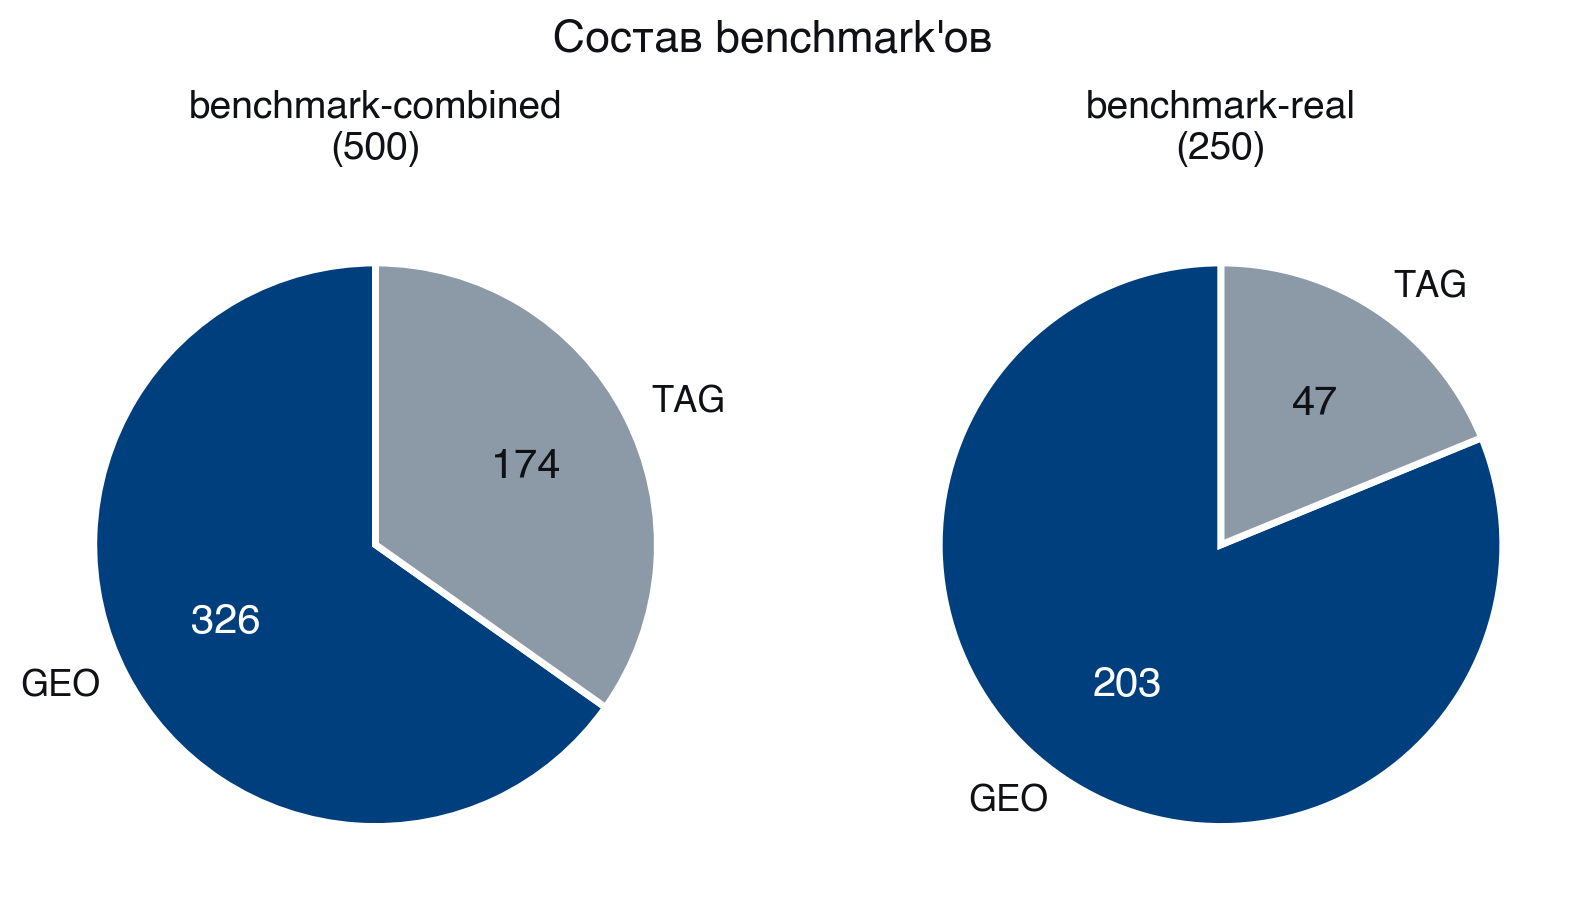
\includegraphics[width=\linewidth]{pictures/benchmark_composition.png}
\end{column}
\begin{column}{0.52\textwidth}
\textbf{Реальные примеры из логов агента:}
\begin{itemize}
  \item \emph{GEO:} «снять квартиру в~центре Казани на~месяц»
  \item \emph{GEO:} «у~метро~Сокол двушку»
  \item \emph{TAG:} «квартира с~панорамными окнами и~видом на~парк»
  \item \emph{TAG:} «у~метро» (категория, без имени)
\end{itemize}

\smallskip
\textbf{Контроль утечек:}\\
500 реальных запросов разделены 50/50 между \texttt{benchmark-real} и \texttt{train-real-250}.\\
Пересечение по нормализованному тексту $= \varnothing$.
\end{column}
\end{columns}
\end{frame}

%% =========================================================
%% 11. Обучающие датасеты
%% =========================================================
\begin{frame}
\frametitle{Обучающие датасеты}
\begin{columns}[T]
\begin{column}{0.5\textwidth}
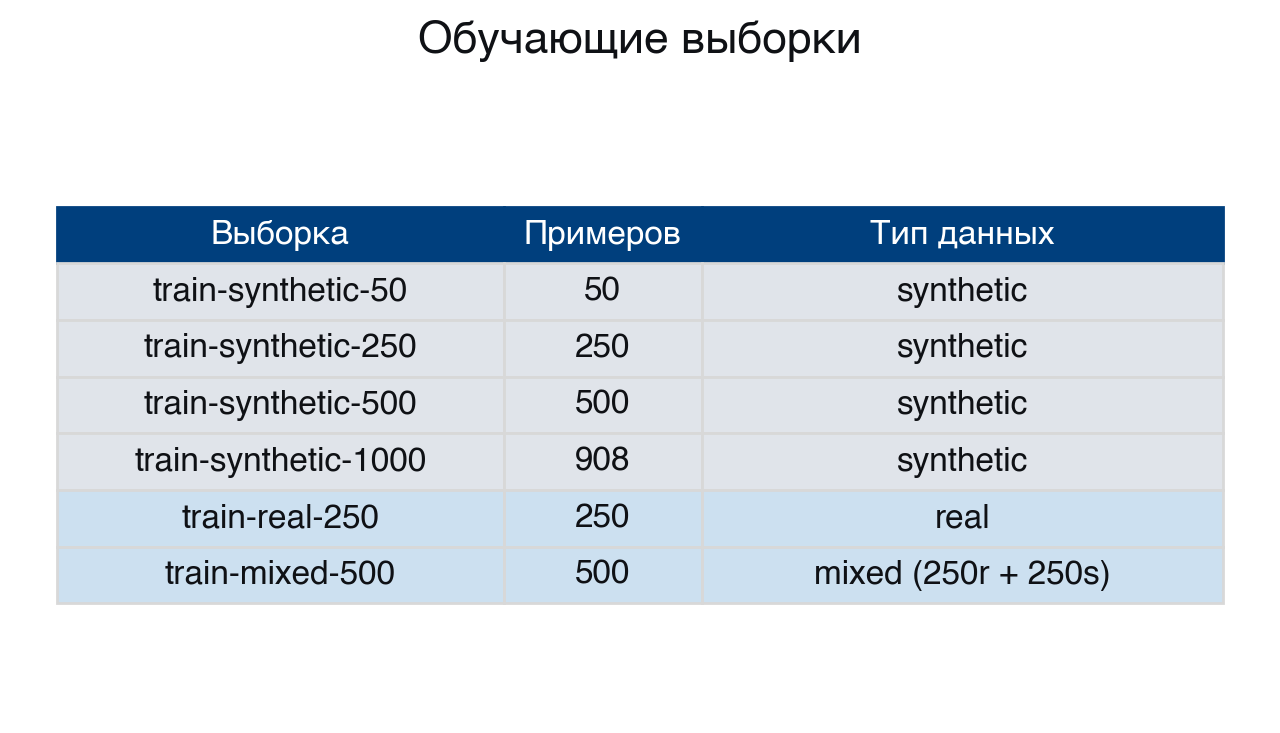
\includegraphics[width=\linewidth,height=0.6\textheight,keepaspectratio]{pictures/training_sets.png}
\end{column}
\begin{column}{0.47\textwidth}
\textbf{6 основных конфигураций:}
\begin{itemize}
  \item \texttt{synth-50/250/500/908}
  \item \texttt{real-250}
  \item \texttt{mixed-500} (250r + 250s)
\end{itemize}

\textbf{+5 итеративных версий:} \texttt{lite\_latest\_v\{1,2,3\}}, \texttt{lite\_rc\_v\{1,2\}}~— $\sim$1500 синтетических примеров.
Корпуса различаются после дедупликации; включены как ablation на устойчивость, не как независимые конфигурации.

\smallskip
Синтетика проходит \textbf{гуманизацию}~— повторный прогон через LLM для сближения со стилем реальных запросов.
\end{column}
\end{columns}
\end{frame}

%% =========================================================
%% 12. Статистический протокол
%% =========================================================
\begin{frame}
\frametitle{Статистический протокол}
\begin{itemize}
  \item \textbf{Глобальный тест.} Cochran~$Q$ ($k = 12$):
  \[
    Q = \frac{k(k-1)\sum_j (T_j - \bar T)^2}{k\sum_i R_i - \sum_i R_i^2} \xrightarrow{d} \chi^2(k - 1)
  \]
  \item \textbf{Попарное сравнение.} Точный McNemar по $\binom{12}{2} = 66$ парам.
  \item \textbf{Поправка Бонферрони:} $\alpha_{\mathrm{adj}} = 0{,}05/66 \approx 0{,}0008$.
  \item \textbf{Доверительные интервалы.} Bootstrap ($B = 1000$, $\mathrm{seed} = 42$), 95\,\%-перцентильный метод.
  \item \textbf{Воспроизводимость.} Фиксированные seed, идентификаторы чекпоинтов в Yandex Cloud, единые бенчмарки без ресемплирования.
\end{itemize}
\end{frame}

%% =========================================================
%% 13. Главное сравнение моделей
%% =========================================================
\begin{frame}
\frametitle{Главное сравнение: 12 моделей на benchmark-combined}
\begin{center}
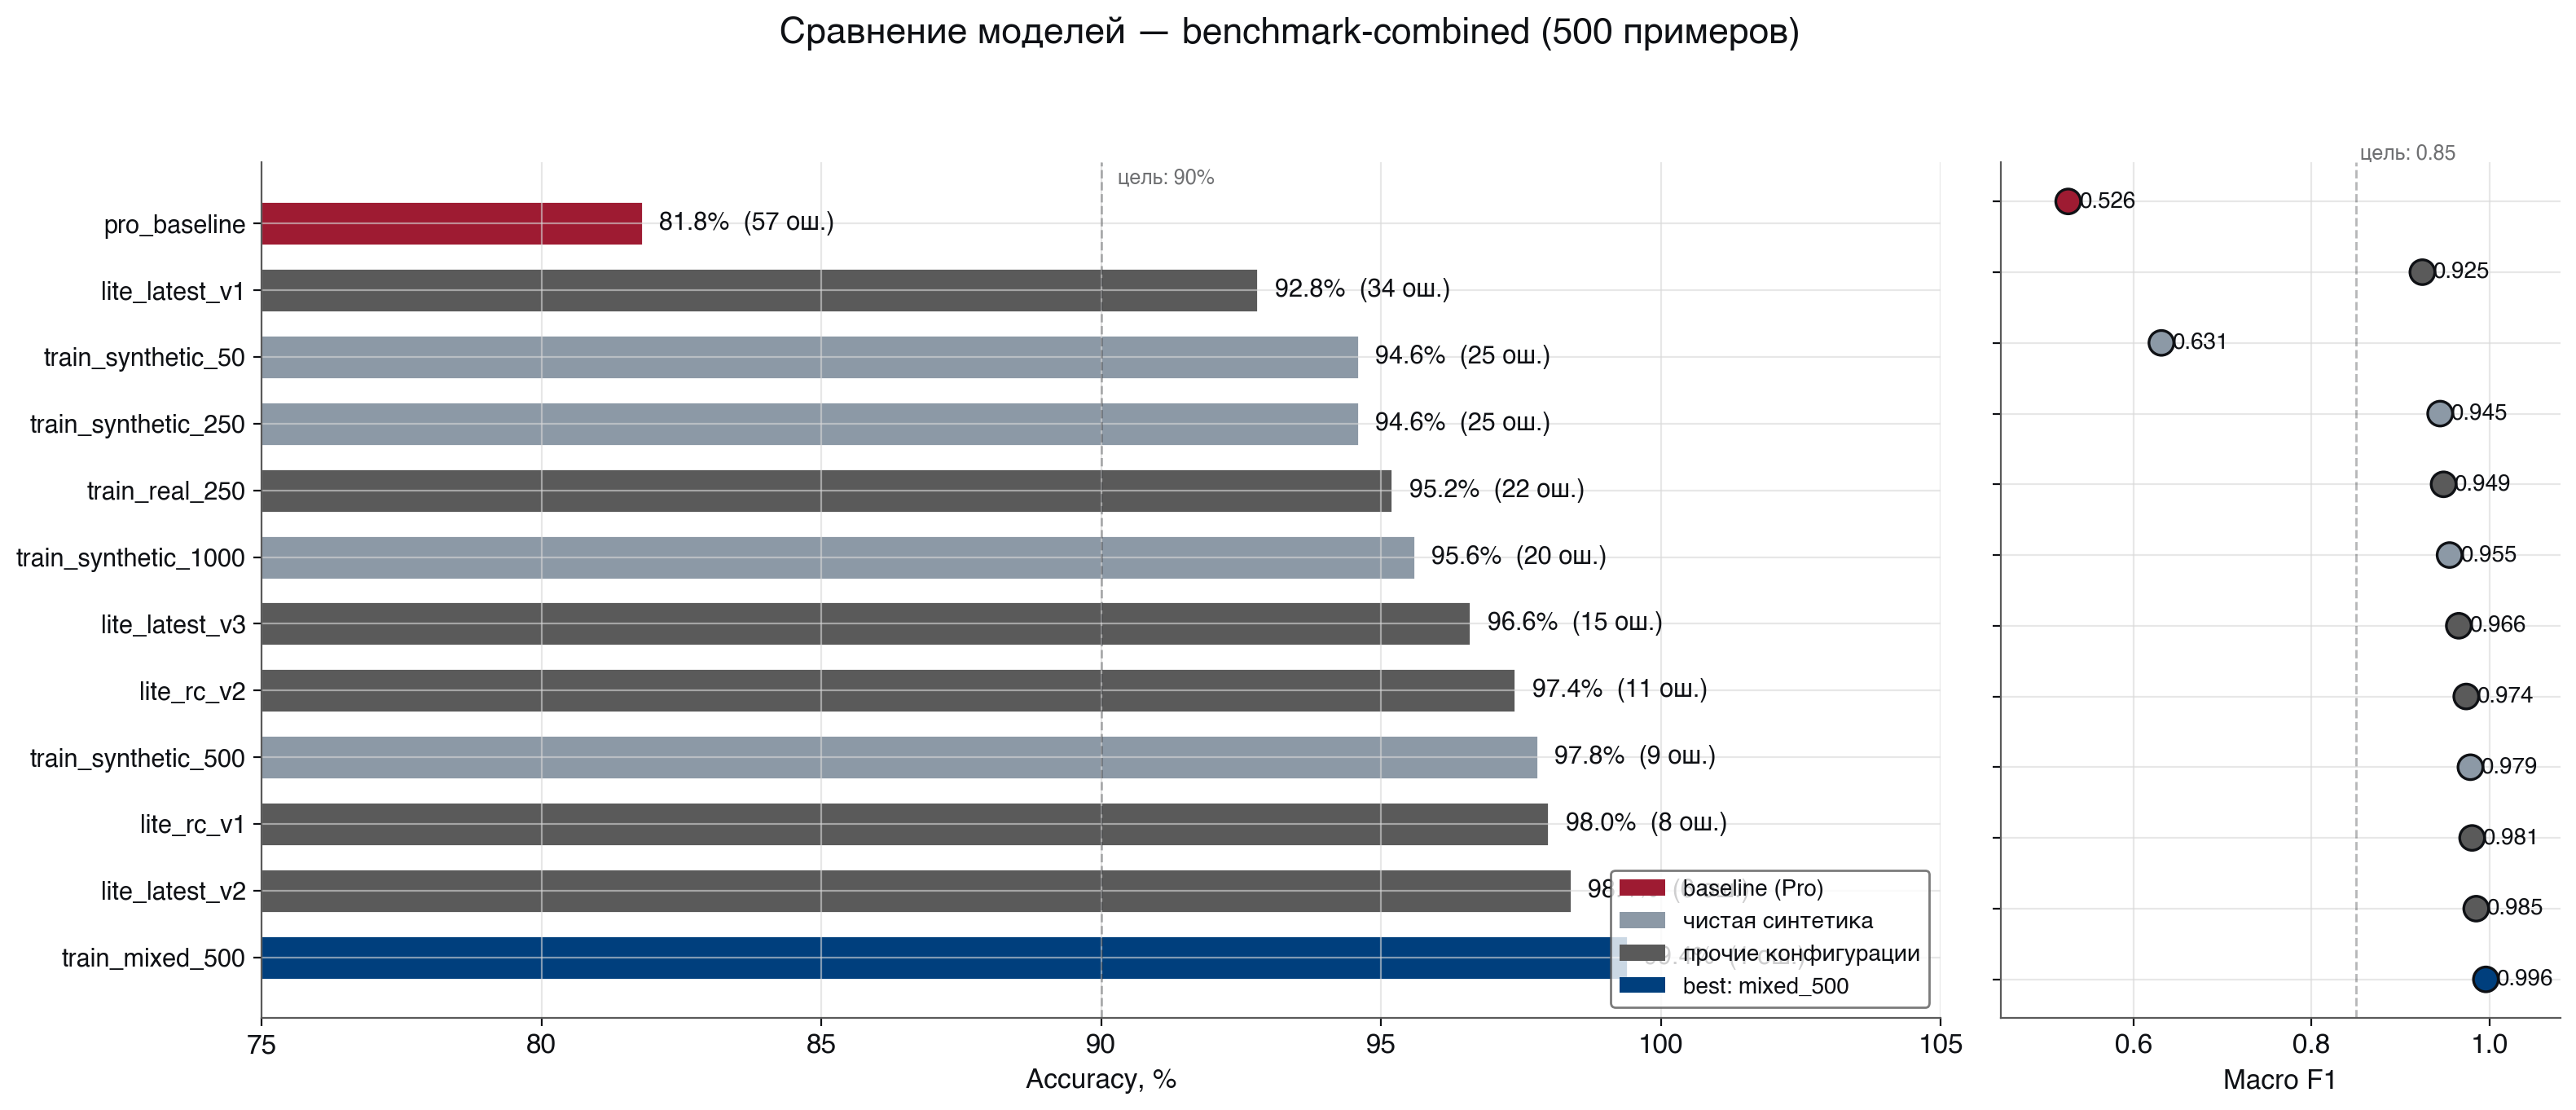
\includegraphics[width=0.85\linewidth,height=0.78\textheight,keepaspectratio]{pictures/model_comparison.png}
\end{center}
\vspace{-0.5em}
{\small \textbf{Чемпион~— \texttt{train\_mixed\_500}:} accuracy $99{,}4\%$, Macro $F_1 = 0{,}996$, 1 ошибка / 500. $\rho_\varnothing$: $6{,}8\% \to 0{,}4\%$.}
\end{frame}

%% =========================================================
%% 14. Кривая насыщения
%% =========================================================
\begin{frame}
\frametitle{Кривая насыщения: synthetic vs mixed}
\begin{center}
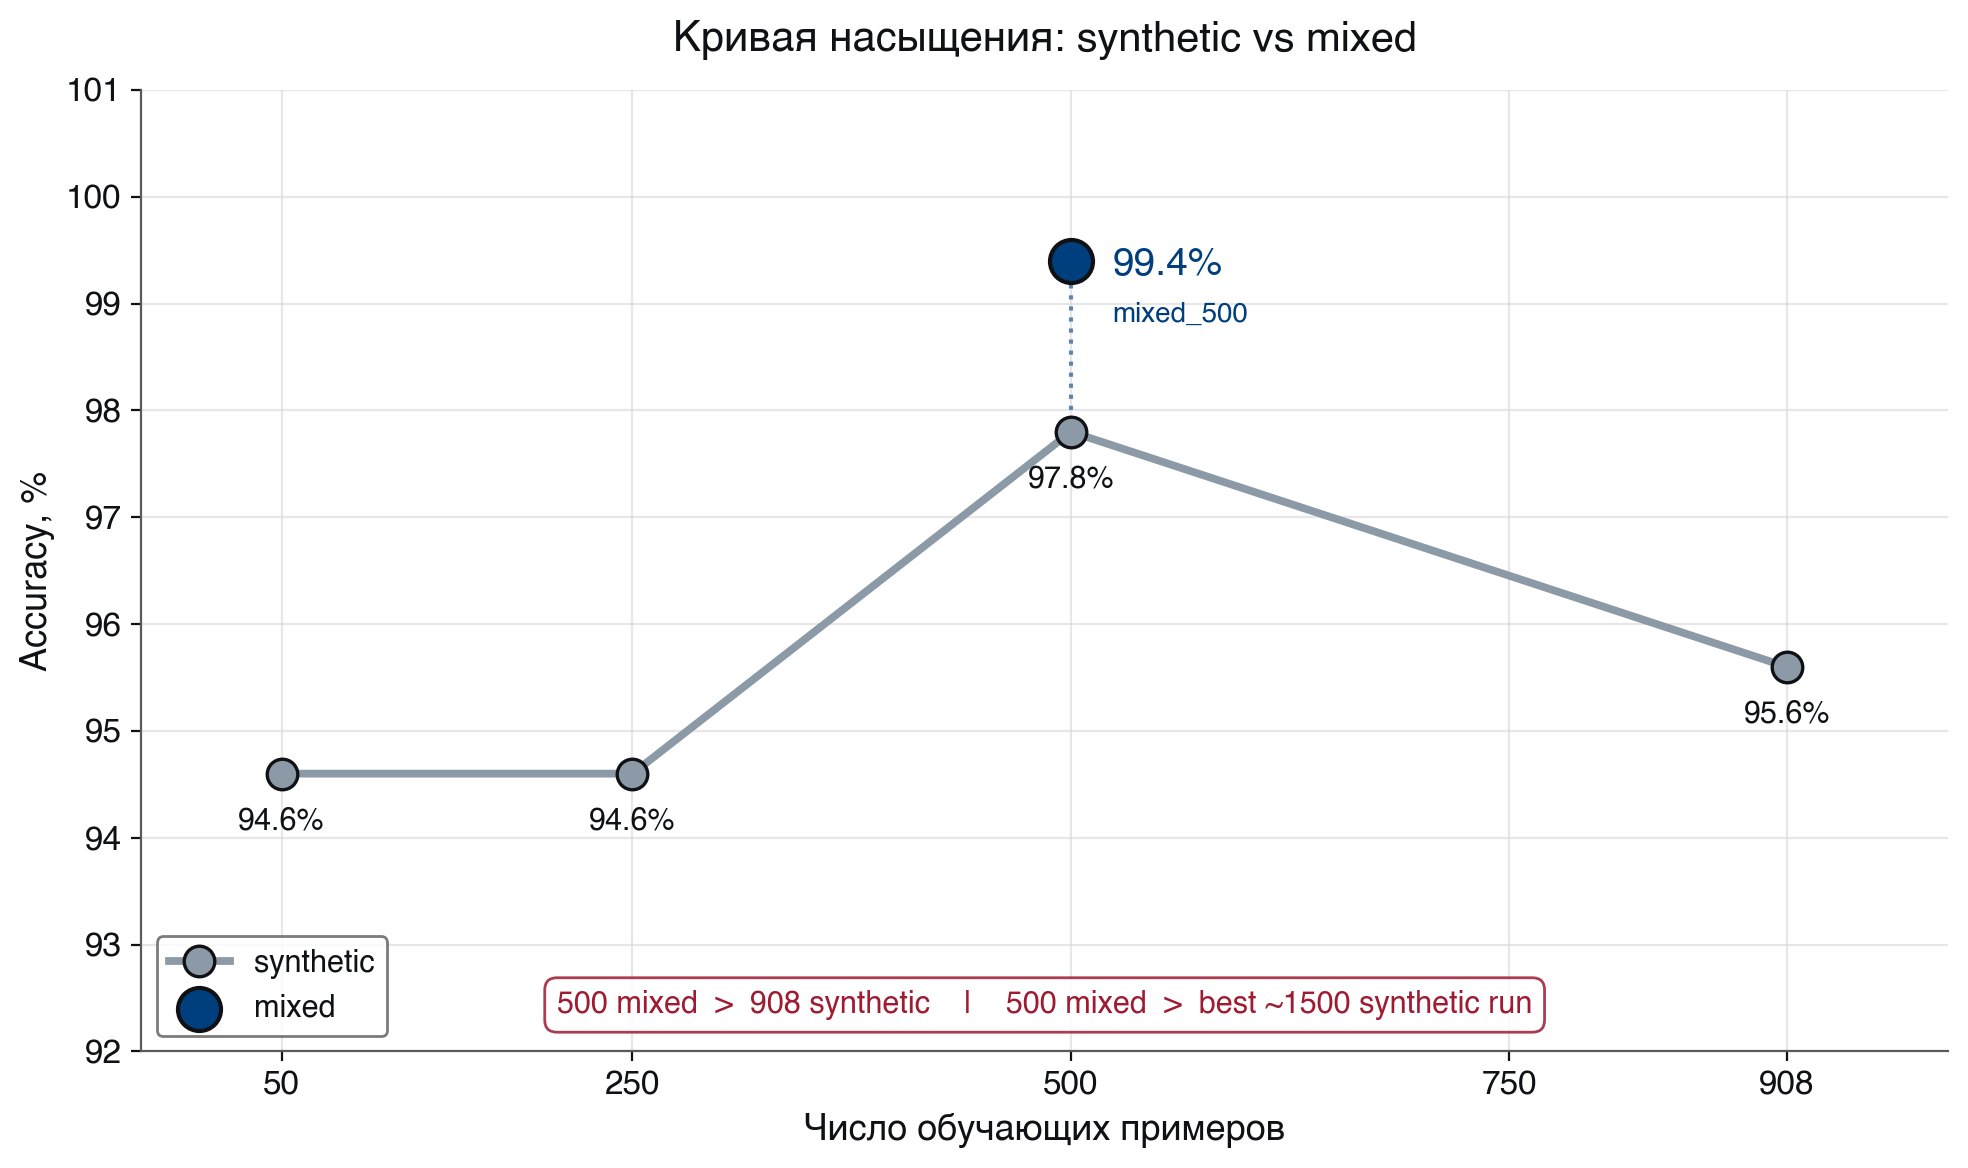
\includegraphics[width=0.7\linewidth,height=0.72\textheight,keepaspectratio]{pictures/saturation_curve.png}
\end{center}
\vspace{-0.6em}
{\small Синтетика: пик $97{,}8\%$ на 500, деградация на 908. \quad
500 mixed $>$ 908 synthetic $>$ best $\sim$1500 synthetic run.}
\end{frame}

%% =========================================================
%% 15. Generalization gap
%% =========================================================
\begin{frame}
\frametitle{Generalization gap: combined $\to$ real}
\begin{center}
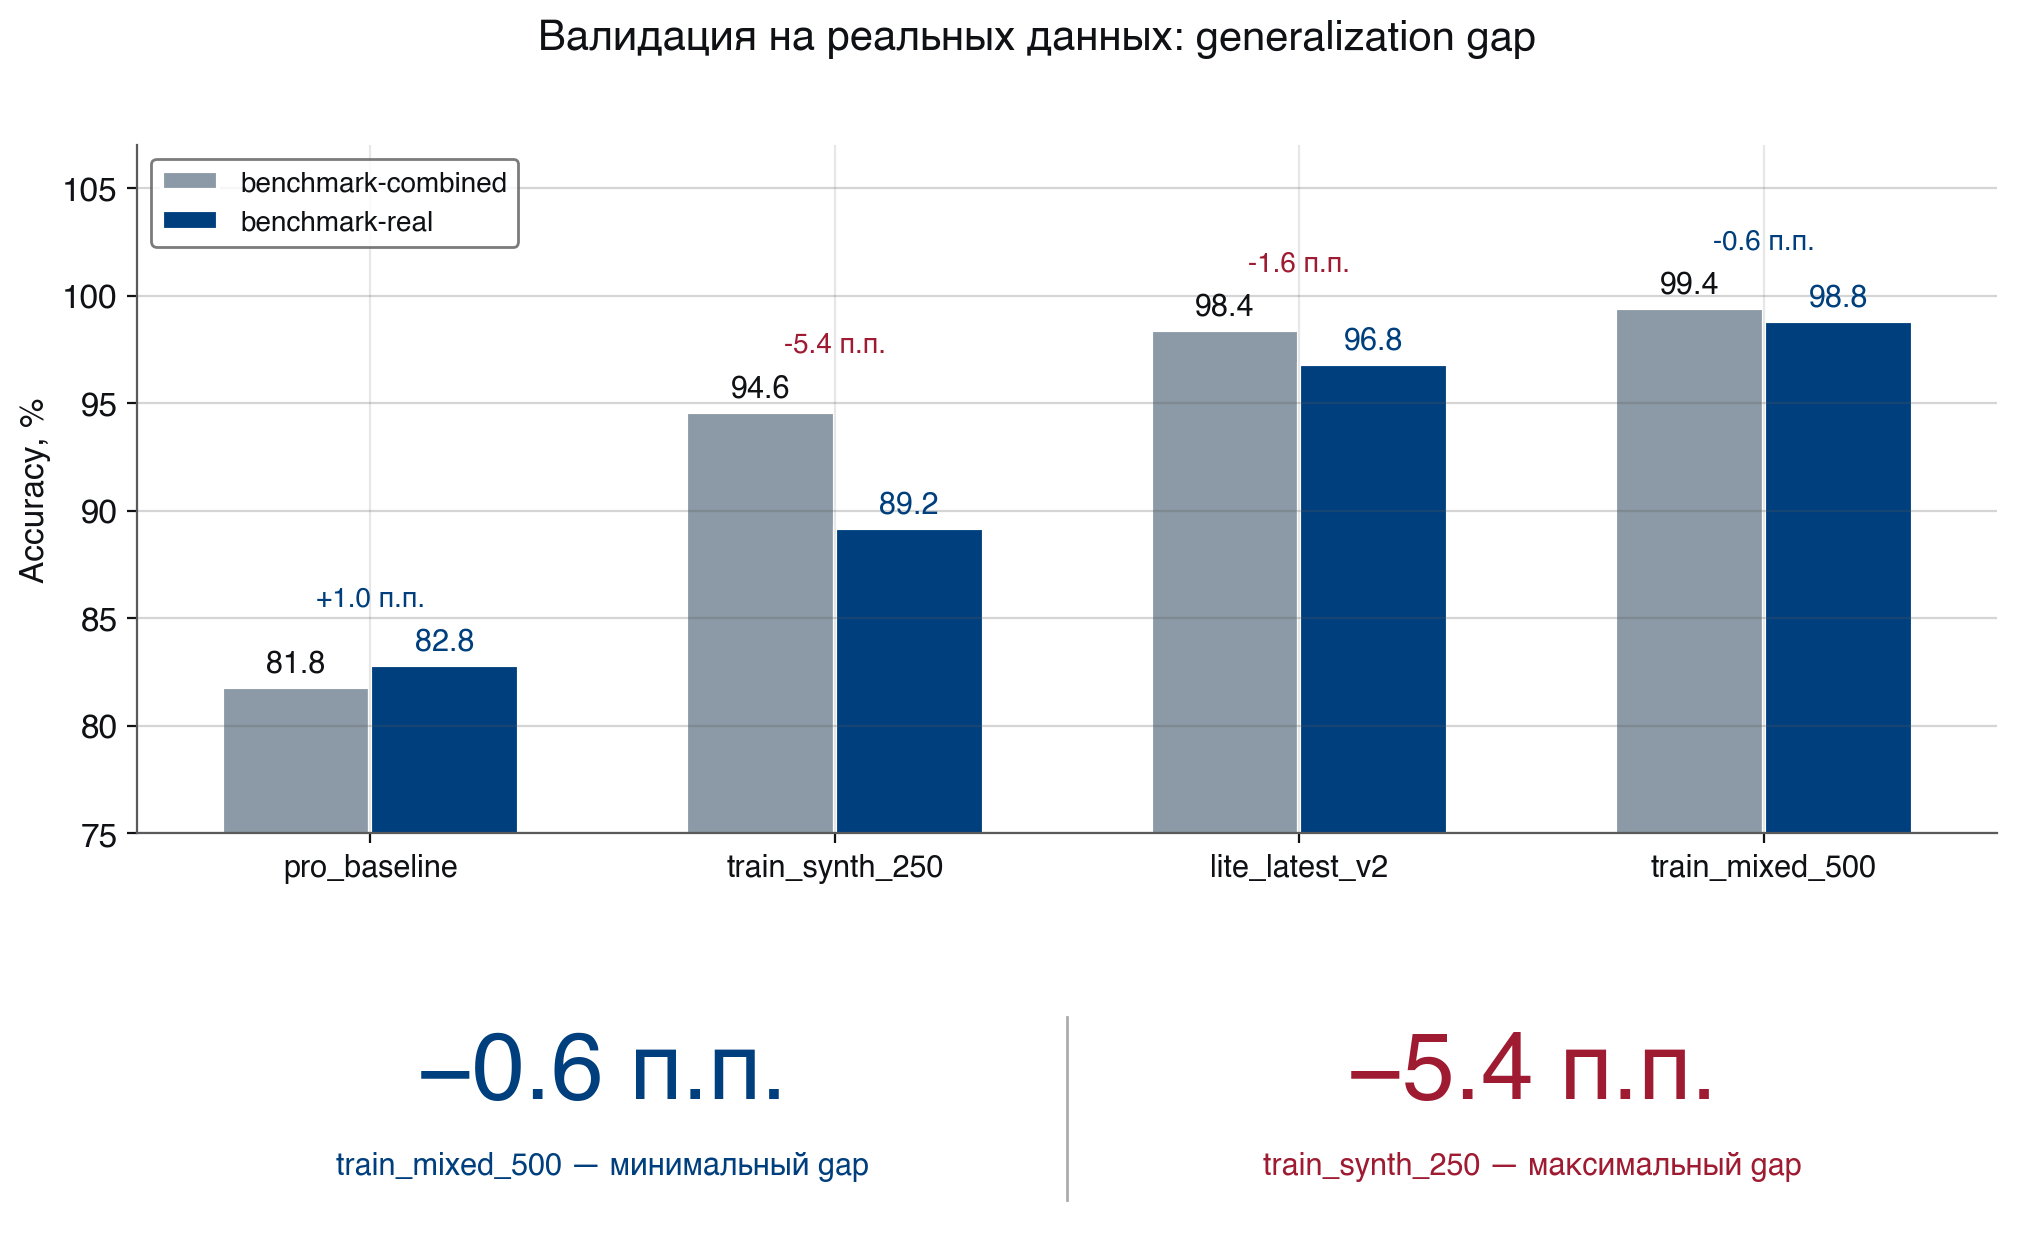
\includegraphics[width=0.78\linewidth,height=0.74\textheight,keepaspectratio]{pictures/generalization_gap.png}
\end{center}
\vspace{-0.5em}
{\small Чисто синтетика теряет $-2{,}2\ldots-5{,}4$~п.п.; \texttt{train\_mixed\_500}~— минимум $-0{,}6$~п.п.\ ($98{,}8\%$).}
\end{frame}

%% =========================================================
%% 16. Аномалия train_synth_50
%% =========================================================
\begin{frame}
\frametitle{Аномалия train\_synth\_50: «паразитный» класс}
\begin{columns}[T]
\begin{column}{0.6\textwidth}
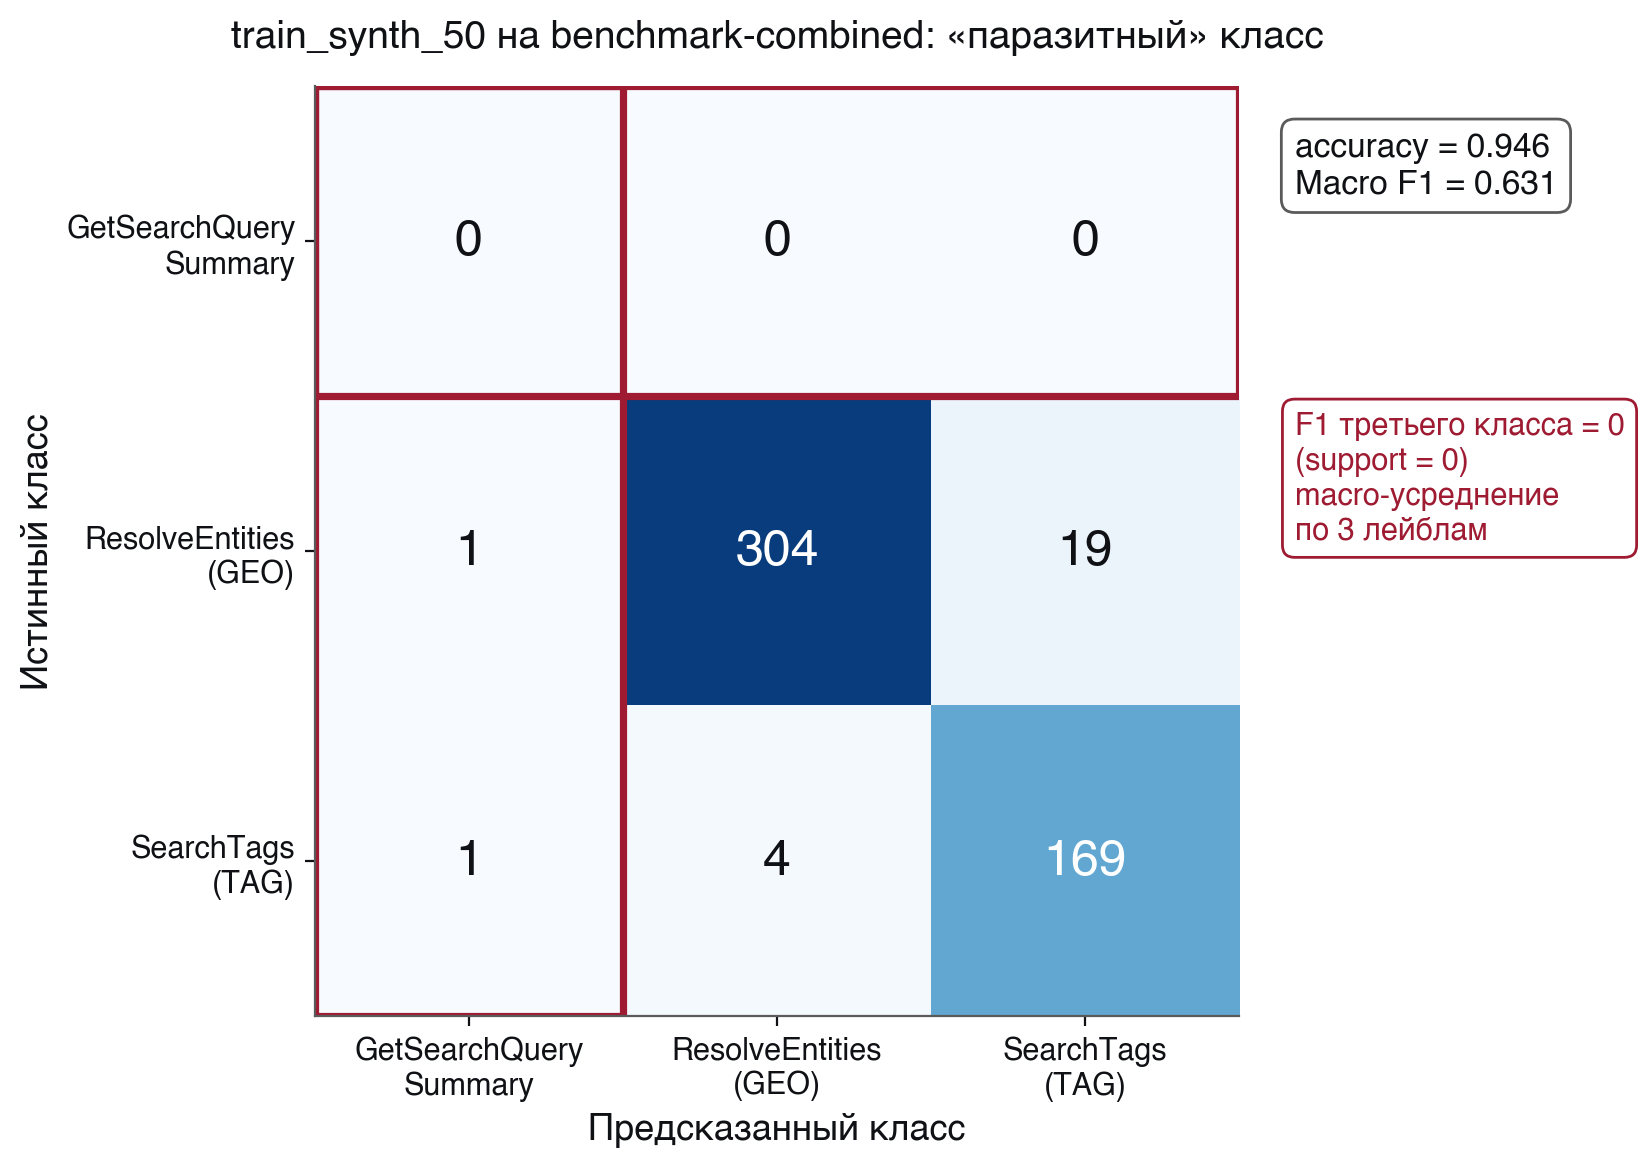
\includegraphics[width=\linewidth]{pictures/parasitic_class.png}
\end{column}
\begin{column}{0.38\textwidth}
\textbf{Внешне противоречие:}\\
accuracy $= 0{,}946$, но Macro $F_1 = 0{,}631$.

\smallskip
\textbf{Объяснение:}\\
модель в 2 случаях из 500 предсказывает несуществующий tool \texttt{GetSearchQuerySummary}.\\
$F_1$ для класса с \texttt{support}$=0$ равен 0; macro-усреднение по 3 лейблам тянет результат вниз.

\smallskip
На 250 примерах паразитный класс исчезает, $F_1$ восстанавливается до $0{,}945$.
\end{column}
\end{columns}
\end{frame}

%% =========================================================
%% 17. Анализ ошибок: инверсия bias
%% =========================================================
\begin{frame}
\frametitle{Анализ ошибок: инверсия bias после дообучения}
\begin{center}
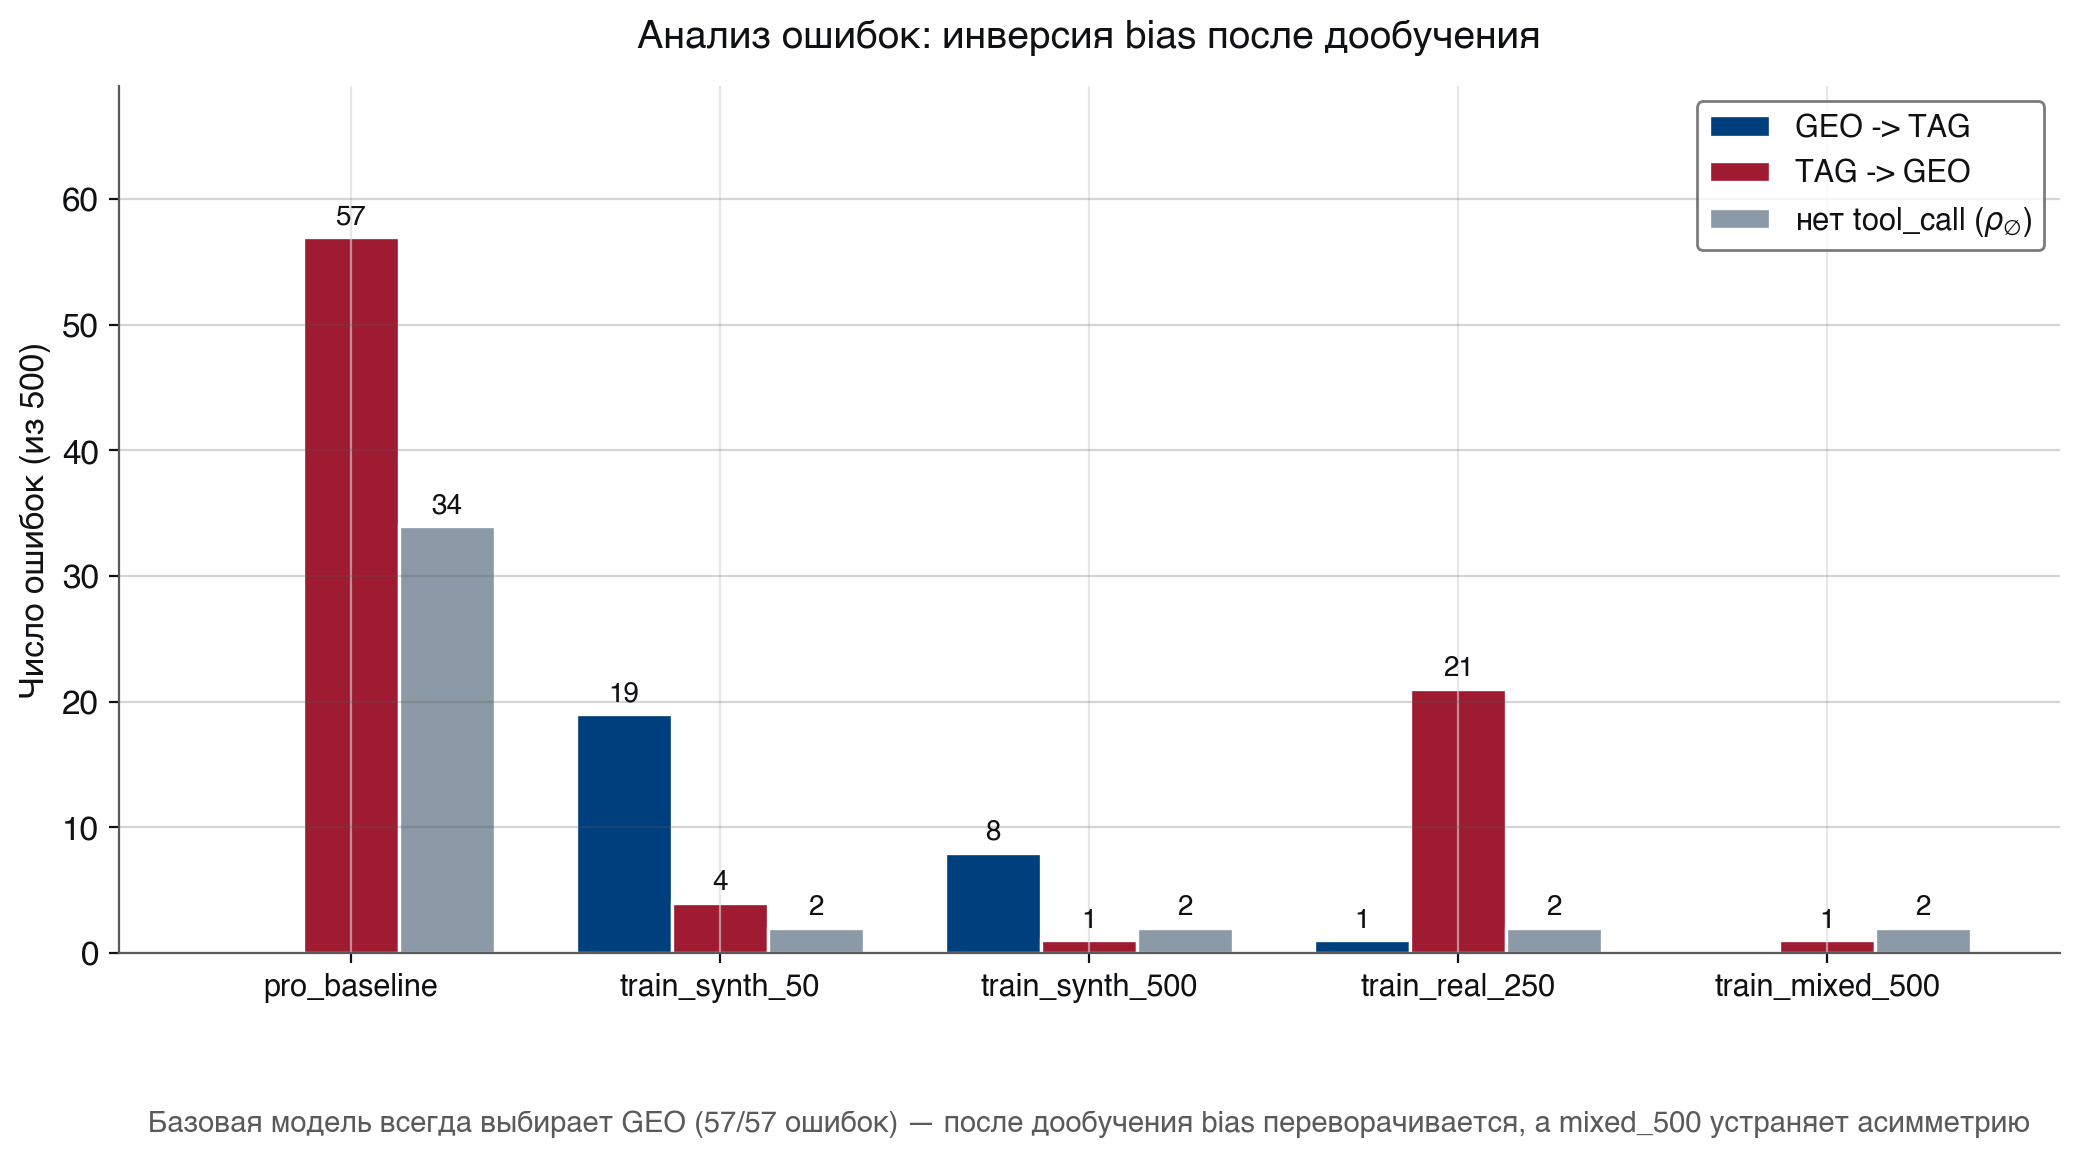
\includegraphics[width=0.72\linewidth,height=0.7\textheight,keepaspectratio]{pictures/error_breakdown.png}
\end{center}
\vspace{-0.5em}
{\small Baseline: 57/57 ошибок $\mathrm{TAG}\!\to\!\mathrm{GEO}$.\\После synth-обучения bias \emph{переворачивается}. Mixed-500: 0 + 1.}
\end{frame}

%% =========================================================
%% 18. Консервация ошибок
%% =========================================================
\begin{frame}
\frametitle{Консервация ошибок: «трудное ядро»}
\begin{columns}[T]
\begin{column}{0.6\textwidth}
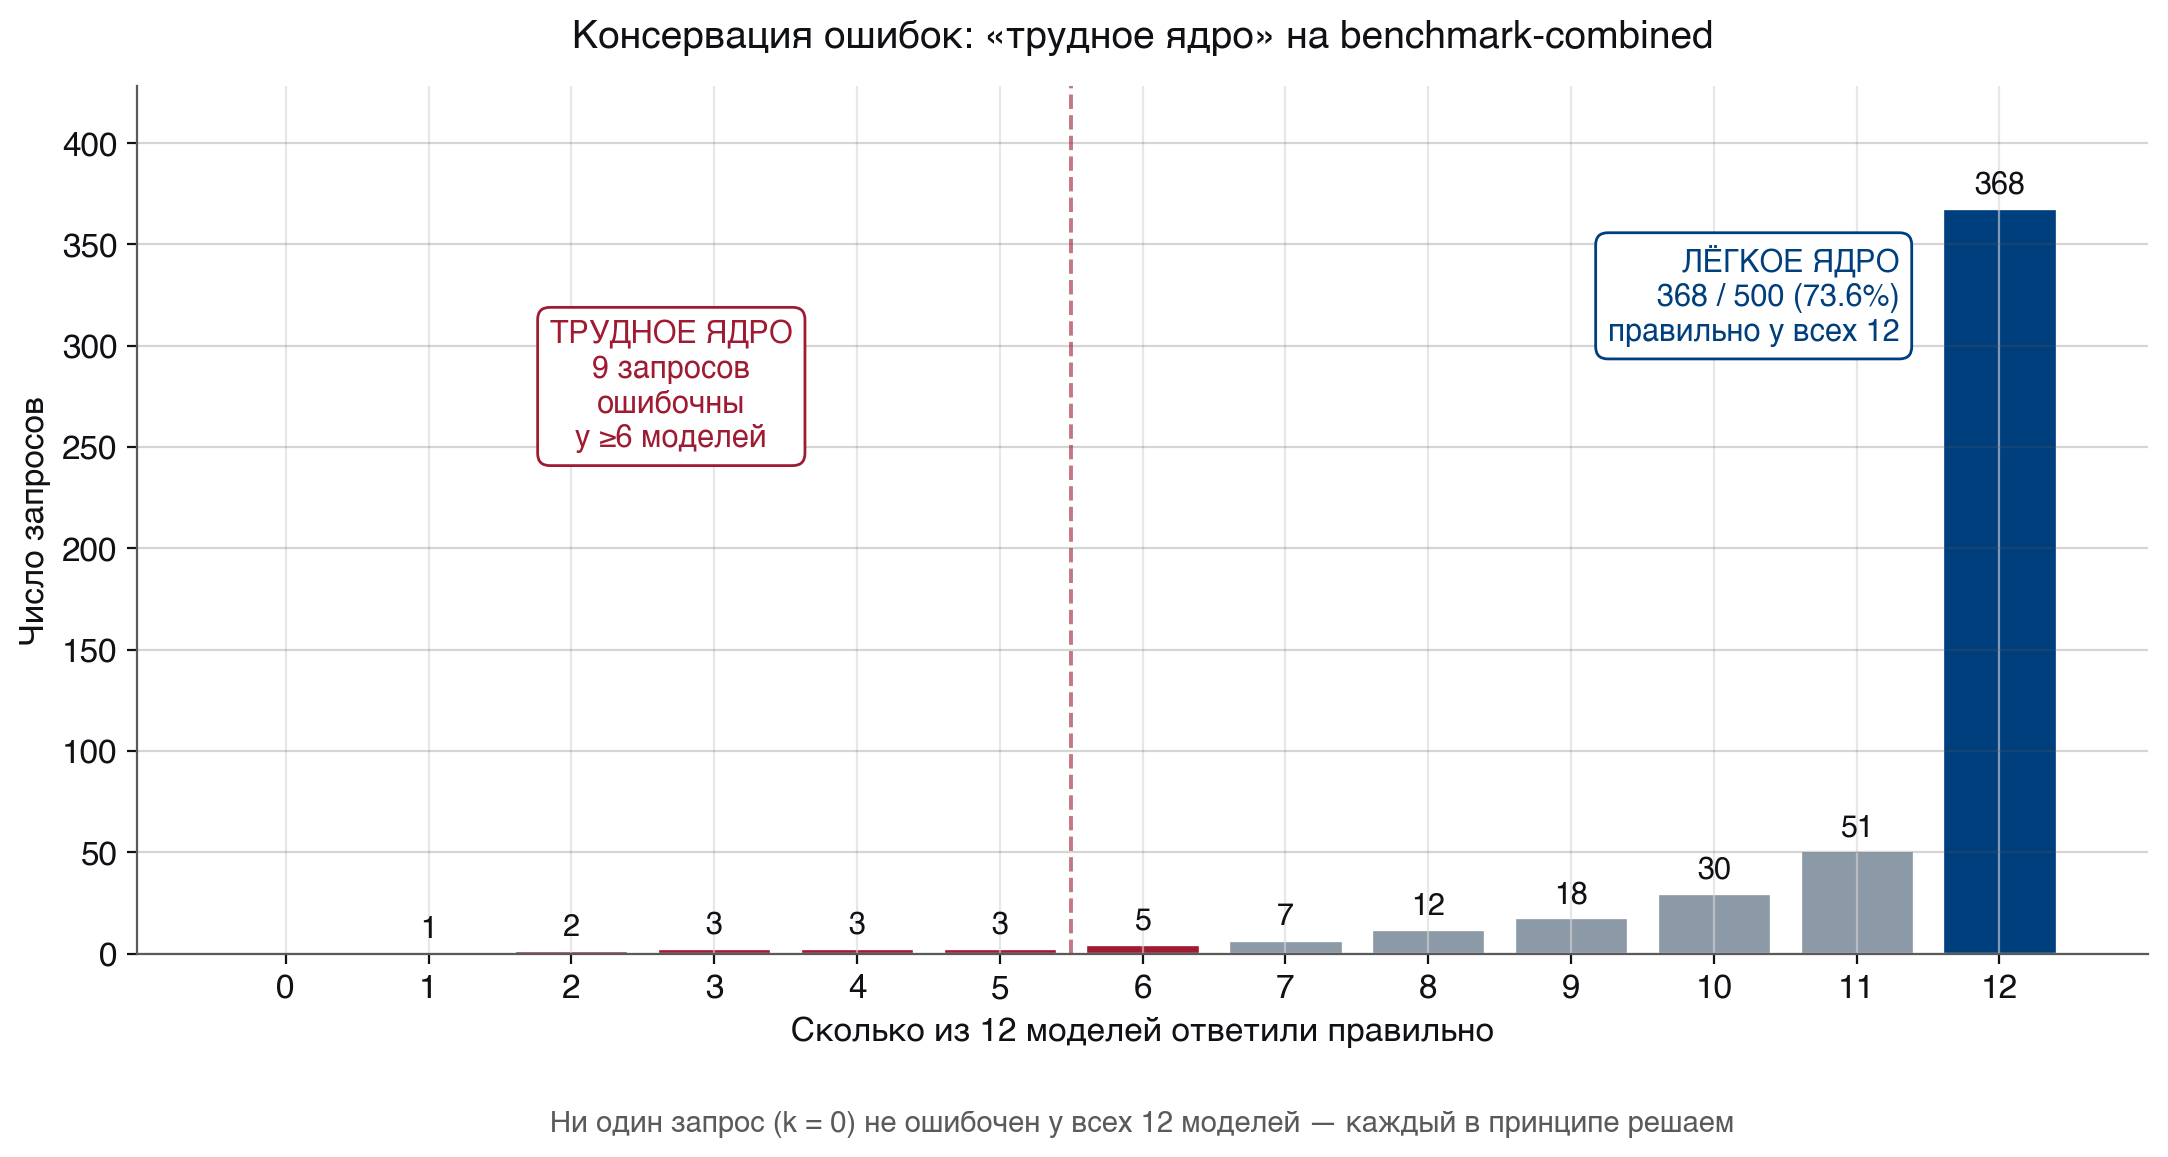
\includegraphics[width=\linewidth,height=0.78\textheight,keepaspectratio]{pictures/error_conservation.png}
\end{column}
\begin{column}{0.38\textwidth}
\textbf{Статистика по 12 моделям:}
\begin{itemize}
  \item $368/500$ ($73{,}6\%$)~— правильно у всех 12;
  \item 0 запросов ошибочны у всех 12 ($\Rightarrow$ каждый в~принципе решаем);
  \item 9 запросов~— у $\geq 6$ моделей.
\end{itemize}

\smallskip
\textbf{Примеры «трудного ядра»:}
\begin{itemize}
  \item «возле зелёной ветки»
  \item «у~ТТК ищу студию»
  \item длинные запросы со смешанной геогр.\,+ тег-семантикой
\end{itemize}
\end{column}
\end{columns}
\end{frame}

%% =========================================================
%% 19. Статистическая значимость
%% =========================================================
\begin{frame}
\frametitle{Статистическая значимость различий}
\begin{columns}[T]
\begin{column}{0.58\textwidth}
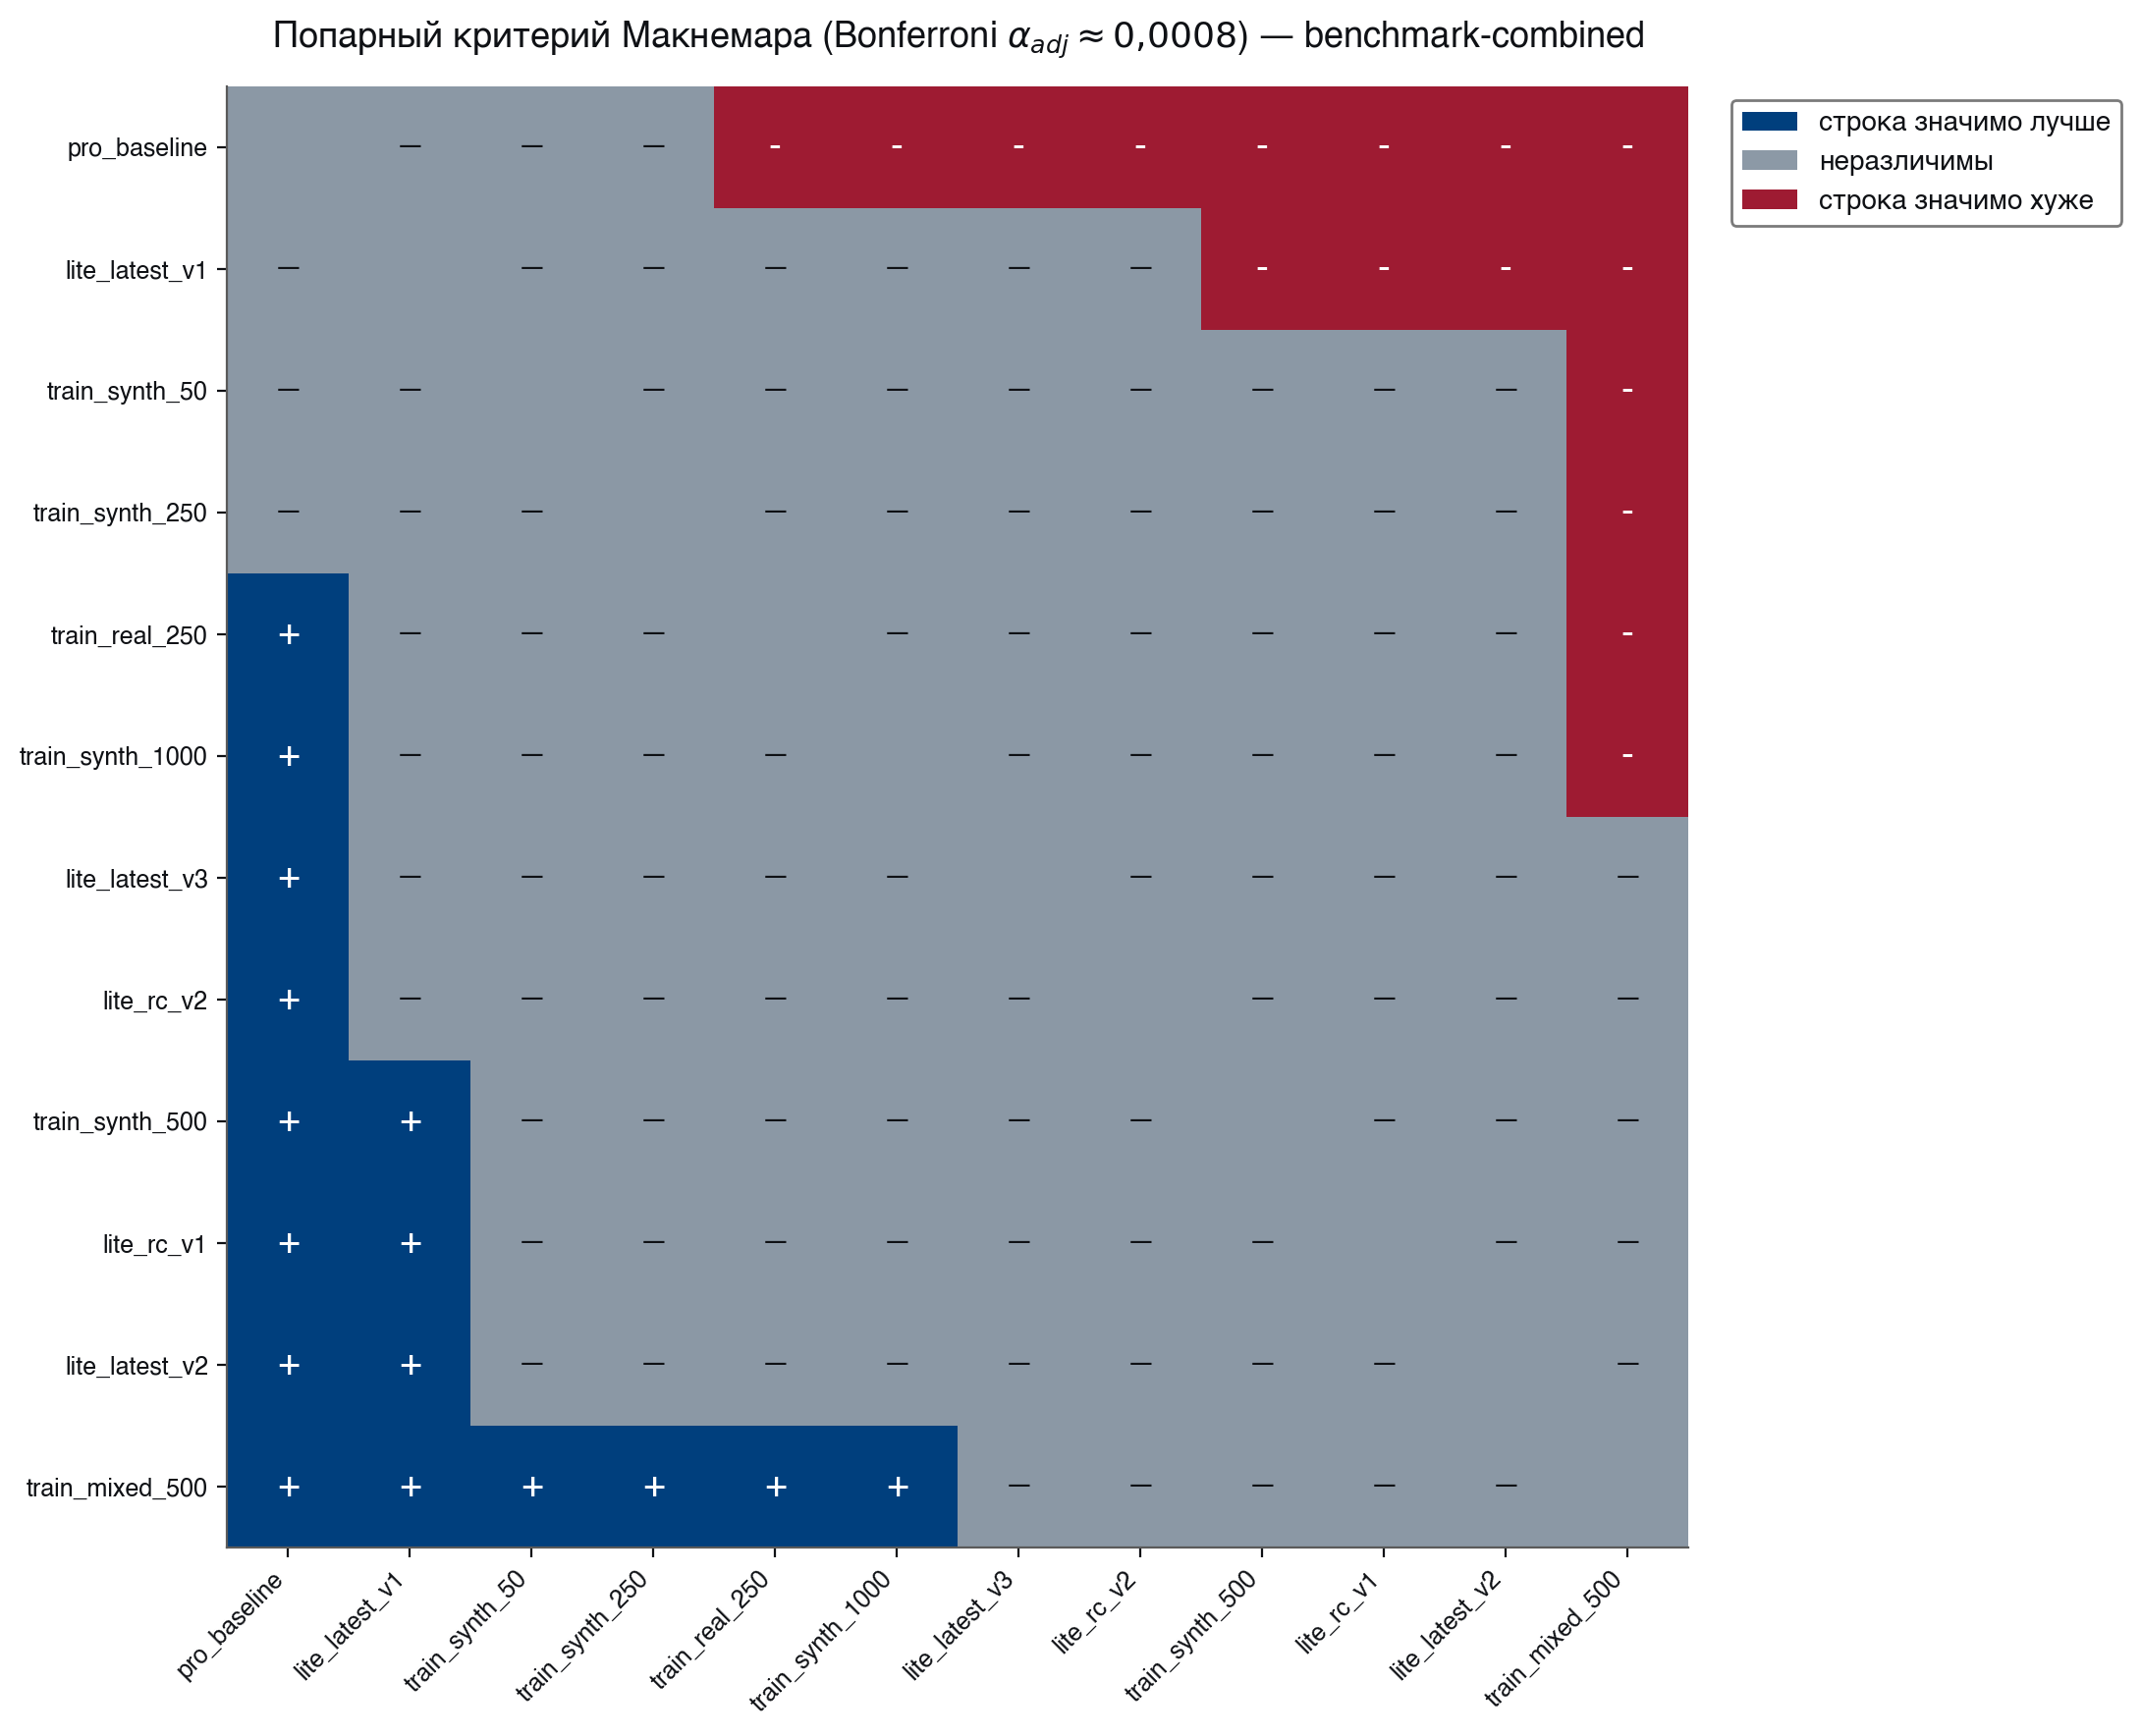
\includegraphics[width=\linewidth,height=0.8\textheight,keepaspectratio]{pictures/mcnemar_heatmap.png}
\end{column}
\begin{column}{0.4\textwidth}
\textbf{Cochran~$Q$:}
\begin{itemize}
  \item combined: $Q = 348{,}0$
  \item real: $Q = 128{,}8$
  \item $p < 10^{-6}$ на обоих
\end{itemize}

\textbf{Попарный McNemar:}
\begin{itemize}
  \item \texttt{mixed\_500} значимо превосходит большинство моделей.
  \item Неразличимо: \texttt{lite\_latest\_v2} ($p = 0{,}73$), \texttt{train\_real\_250} ($p = 0{,}50$).
  \item Все чисто синтетические значимо уступают на benchmark-real.
\end{itemize}
\end{column}
\end{columns}
\end{frame}

%% =========================================================
%% 20. Bootstrap-CI accuracy на real
%% =========================================================
\begin{frame}
\frametitle{Bootstrap-CI accuracy на benchmark-real}
\begin{center}
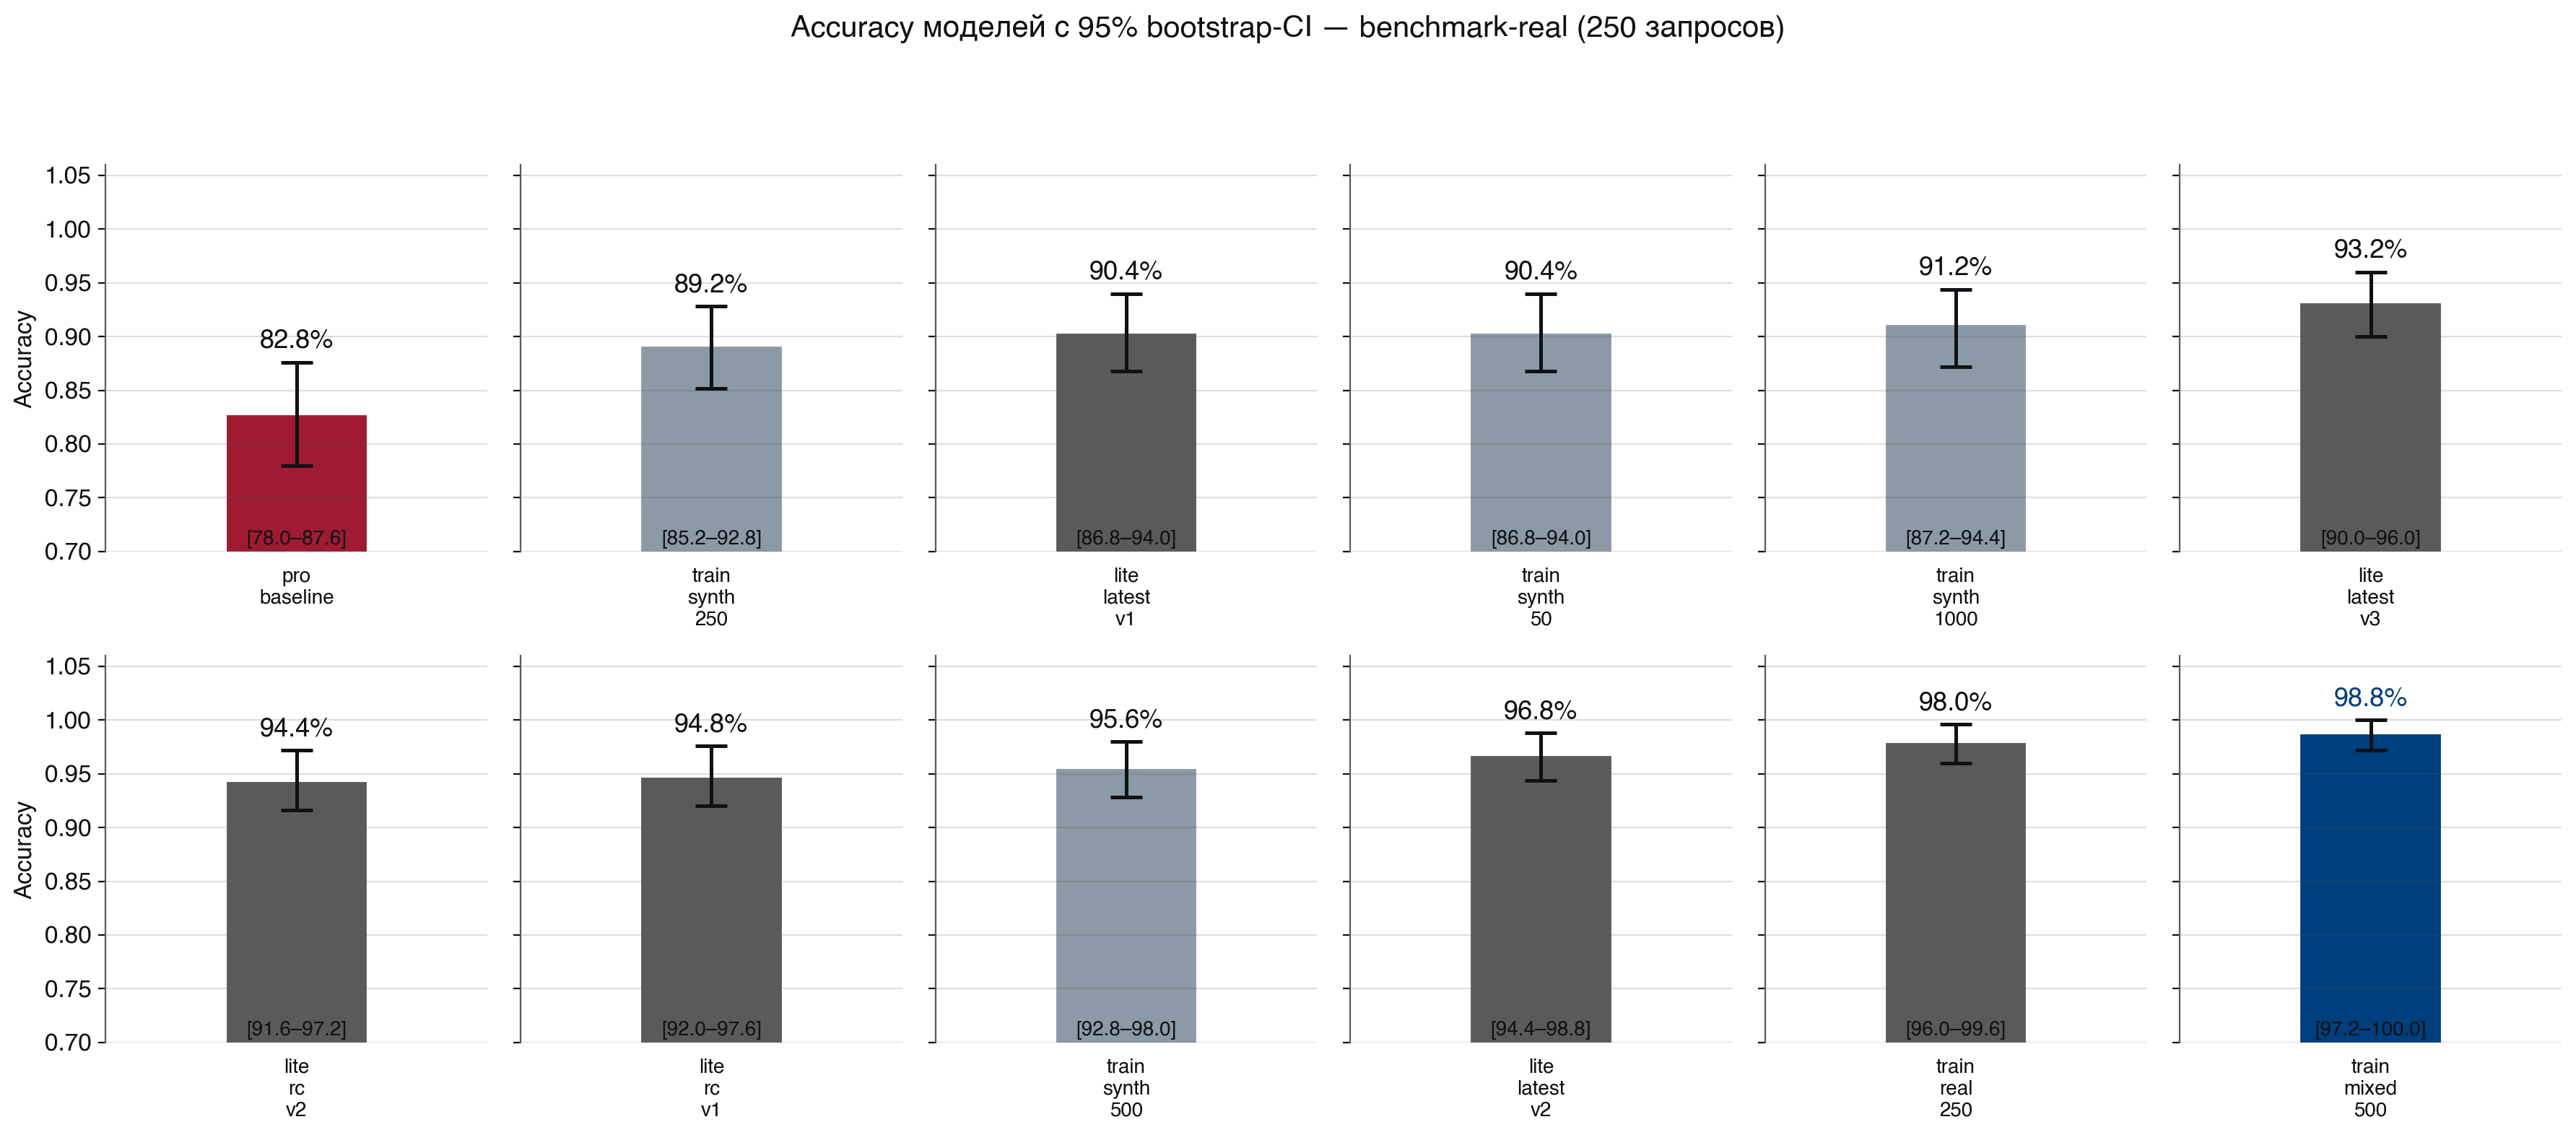
\includegraphics[width=0.85\linewidth,height=0.78\textheight,keepaspectratio]{pictures/accuracy_ci.png}
\end{center}
\vspace{-0.5em}
{\small H1b подтверждена: нижняя граница CI \texttt{train\_mixed\_500} $= 0{,}972 > 0{,}90$.}
\end{frame}

%% =========================================================
%% 21. Ответы на исследовательские вопросы
%% =========================================================
\begin{frame}
\frametitle{Ответы на исследовательские вопросы}
\begin{description}
  \item[\textsc{RQ1.}] LoRA-дообучение поднимает accuracy с $81{,}8\%$ до $99{,}4\%$ ($+17{,}6$~п.п.); все различия значимы.
  \item[\textsc{RQ2.}] Зависимость немонотонна: 50 примеров уже дают $94{,}6\%$, пик на 500 синтетике, деградация на 908.
  \item[\textsc{RQ3.}] Тип данных решает: чисто синтетика теряет до $-5{,}4$~п.п.\ на real; mixed-стратегия даёт $-0{,}6$.
  \item[\textsc{RQ4.}] H1a, H1b, H2~— подтверждены строгими тестами.
\end{description}
\end{frame}

%% =========================================================
%% 22. Переносимый рецепт + threats to validity
%% =========================================================
\begin{frame}
\frametitle{Переносимый рецепт и угрозы валидности}
\begin{columns}[T]
\begin{column}{0.52\textwidth}
\textbf{Рецепт адаптации AI-агента:}
\begin{enumerate}
  \item $N$ реальных + $M$ синтетических примеров с балансом $\sim$50/50.
  \item LoRA малого ранга вместо full fine-tuning.
  \item Обязательная валидация на реальном бенчмарке.
  \item Контроль $\rho_\varnothing$ (отказы вызова инструмента).
\end{enumerate}

\smallskip
\textbf{Область применения:}\\
tool routing в AI-ассистентах, enterprise-агенты, оркестрация API-вызовов.
\end{column}
\begin{column}{0.45\textwidth}
\textbf{Threats to validity:}
\begin{itemize}
  \item Внутренняя: 1 прогон inference, неуправляемые гиперпараметры LoRA.
  \item Внешняя: одно семейство моделей (YandexGPT 5.1), 2 инструмента, узкий домен.
  \item Конструктная: оценивается только первый \texttt{tool\_call}, не аргументы.
  \item Статистическая: Bonferroni консервативна при коррелирующих моделях.
\end{itemize}
\end{column}
\end{columns}
\end{frame}

%% =========================================================
%% 23. Направления развития
%% =========================================================
\begin{frame}
\frametitle{Направления дальнейших исследований}
\begin{itemize}
  \item \textbf{Альтернативные PEFT-методы.} QLoRA, Adapter Tuning против LoRA при равном бюджете данных.
  \item \textbf{Перенос на другие LLM.} GigaChat, Saiga, ruGPT~— проверка универсальности рецепта.
  \item \textbf{Probing-эксперименты.} CKA / linear probes для строгой проверки SAH в decoder-only архитектуре.
  \item \textbf{Масштабирование $|\mathcal{T}| > 2$.} Перенос рецепта на каталог из десятков инструментов.
\end{itemize}
\end{frame}

%% =========================================================
%% 24. Спасибо за внимание
%% =========================================================
{
\setbeamertemplate{footline}{}
\begin{frame}
\begin{center}
{\LARGE \textbf{Спасибо за внимание!}}

\bigskip
{\large Вопросы?}

\bigskip\bigskip
\begin{tabular}{rl}
Студент: & Горошко~А.~В., группа 22.Б13-мм \\
Научный руководитель: & доцент кафедры информатики Григорьева~А.~В. \\
Рецензент: & ст.\,преп.\ кафедры компьютерных технологий\\
 & и систем, к.\,ф.-м.\,н.\ Севостьянов~Р.~А. \\
\end{tabular}

\bigskip
{\scriptsize Санкт-Петербургский государственный университет\\
Кафедра математики и компьютерных наук\\
Санкт-Петербург, 2026}
\end{center}
\end{frame}
}

\end{document}
